\section{Realisierung des neuen Krabbelroboters}
\label{sec:realisierung}

Dieses Kapitel gibt einen kompakten Überblick über die praktische Umsetzung des neuen Krabbelroboters. Die wichtigsten Arbeitsschritte, Herausforderungen und \linebreak Lösungswege von der Übernahme des Legacy-Projekts bis zur Entwicklung der neuen Hardware werden dargestellt.

\subsection{Übernahme des Legacy-Projekts}

Erstes Ziel war zu Projektbeginn, das Vorgängerprojekt zu reaktivieren und zum Laufen zu bekommen. Entsprechende Versuche scheiterten jedoch an unterschiedlichen Faktoren: Der Quellcode des Legacy-Programms war zwar öffentlich auf GitHub synchronisiert, allerdings ohne jegliche Anleitung bezüglich des Programmstarts, benötigter Software-Bibliotheken oder Veränderungen an der Installation des Betriebssystems. Nach mehreren Stunden des Debuggens war der beste Zustand, den wir erreichen konnten, das Programm mit ROS 1 in einem Docker-Image auszuführen. Da die isolierte Container-Umgebung allerdings scheinbar immer noch nicht den nötigen Startbedingungen entsprach, stürzte das Legacy-Programm weiterhin nach Start sofort ab. Nachdem die Arbeit eines ganzen Tages ein so enttäuschendes Ergebnis geliefert hatte, entschieden wir, das Programm von Grund auf neu zu schreiben und dabei den Fokus auf gute Dokumentation des Projekts und eine gute Developer Experience zu legen, um uns selbst sowie möglichen Nachfolgern des Projekt die Arbeit softwareseitig zu erleichtern.

\subsection{Probleme mit dem Raspberry Pi}

Im Zuge des Neuschreibens der Codebase sollte auch die auf dem Raspberry Pi installierte Ubuntu-Version angehoben werden. Als wir allerdings versuchten, den Microcontroller auf dem alten Roboter zu starten, hing dieser stets in einer Boot-Schleife, startete also nicht das Betriebssystem. Nach wiederum einem Tag des Debuggens mit verschiedenen Betriebssystemen, Speichermedien, Netzteilen und Monitorkabeln war mit dem alten Raspberry Pi immer noch kein Betriebbsystem zu starten. Wir kamen zu dem Schluss, dass der spezifische Raspberry Pi auf dem alten Roboter zu Schaden gekommen sein musste, seit wir das letzte Mal damit gearbeitet hatten, vermutlich im Transport. Freundlicherweise konnte uns Prof. Dr. Ihme ein Ersatzmodell aus dem Inventar der Technischen Hochschule Mannheim beschaffen, sodass wir zeitig an dem Projekt weiterarbeiten konnten.

\subsection{Hardware}

Ausgehend von der theoretischen und praktischen Analyse des bestehenden Roboters (siehe Abschnitt~\ref{sec:konzeption}) wurde ein neues mechanisches Konzept für das Chassis des Krabbelroboters 
entwickelt. Ziel war es, die Komponenten platzsparend, gewichtsoptimiert und modular anzuordnen um die Zugänglichkeit zu erweitern.

Zunächst erfolgte eine Recherche der Maße der Bauteile. Auf Basis dieser Daten wurde eine grobe Anordnung in Form einer Handskizze konzipiert, um ein erstes Gefühl für die Platzverhältnisse zu bekommen.

Das daraus abgeleitete 3D-Modell wurde mithilfe von Autodesk Fusion 360 erstellt. Die Konstruktion wurde in zwei funktionale Ebenen aufgeteilt: 
eine untere Ebene zur zur Steuerung der Motoren und eine obere Ebene zur Steuerung der restlichen Bauteile. 
Die Ebenen wurden als separate Körper modelliert, um spätere Anpassungen zu erleichtern.

Der erste 3D-Druck diente zur Kalibrierung der Maße und Überprüfung der Passgenauigkeit. Dabei traten mehrere Fehler auf: 
Einige Schraubenlöcher waren falsch positioniert, die Inkrementalgeber lagen zu nah beieinander, und die Höhe der oberen Griffe erwies sich als zu gering, 
da die Akkumaße zunächst nur geschätzt worden waren.

Da der alte Roboter bis dahin noch softwareseitig genutzt wurde, konnte der mechanische Umbau erst nach Abschluss der entsprechenden Software-Tests (z.\,B. Implementierung des Q-Learnings). 
Anschließend wurde das CAD-Modell überarbeitet und an die gewonnenen Erkenntnisse angepasst.

Der zweite Druckvorgang verlief erfolgreich: Die Bauteile passten wie geplant, alle Komponenten konnten montiert werden. 
Der Aufbau des neuen Roboters war damit abgeschlossen und bildete die Grundlage für die weitere softwareseitige Integration.
Abbildung~\ref{fig:crawler_side} zeigt den Krabbelroboter in der Seitenansicht zum Projektabschluss.

\begin{figure}[H]
    \centering
    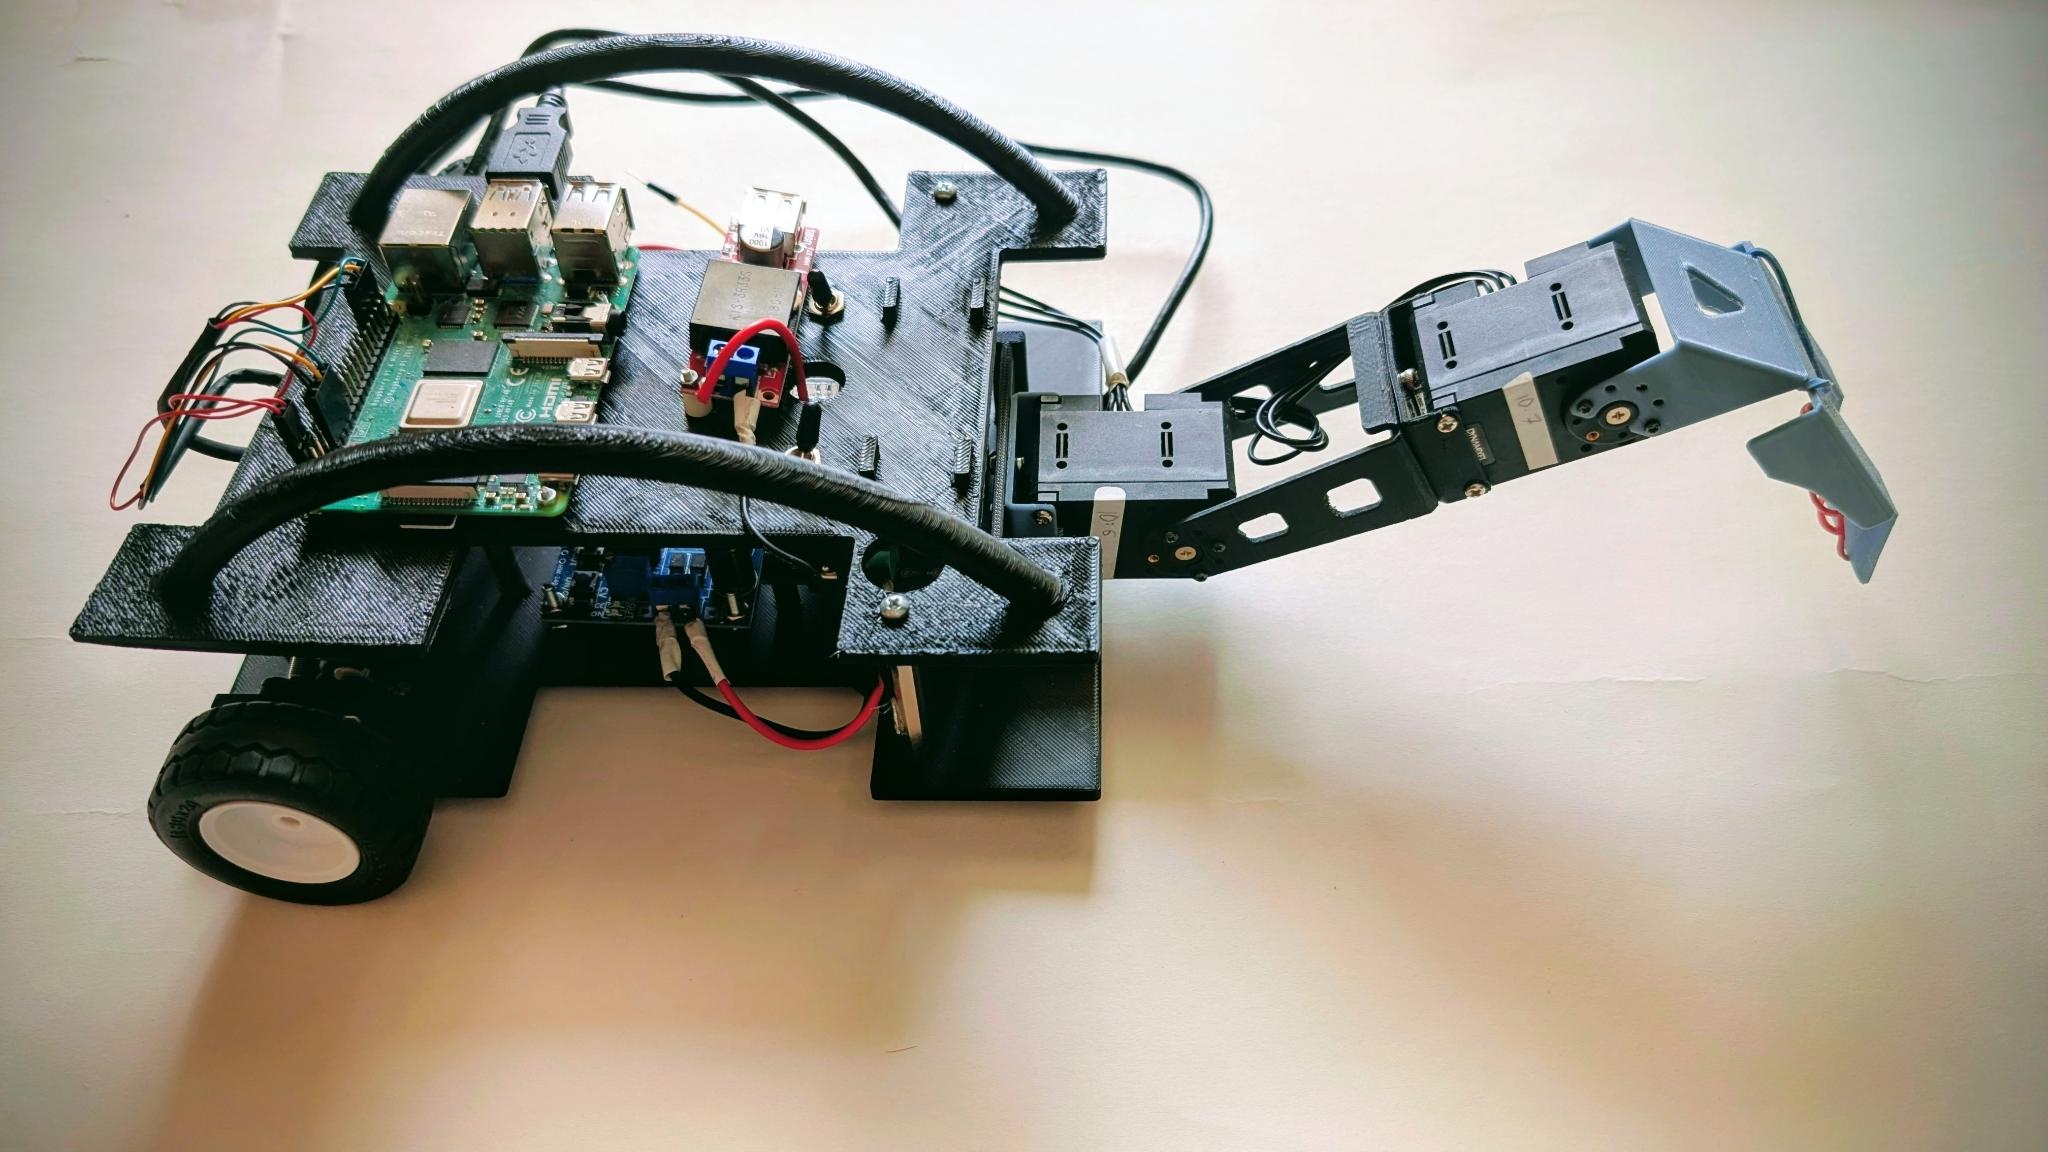
\includegraphics[width=0.8\textwidth]{crawler_side.jpeg}
    \caption{Seitliche Ansicht des Krabbelroboters zum Projektabschluss.}
    \label{fig:crawler_side}
\end{figure}
